\documentclass[12pt,a4paper]{article}
%\usepackage{babel}
\usepackage[utf8]{inputenc}
\usepackage[french]{babel}
\usepackage{amsmath}
\usepackage{amsfonts}
\usepackage{amssymb}
\usepackage{makeidx}
\usepackage{graphicx}
\usepackage{enumerate}
\usepackage{pdfpages}
\usepackage{cite}
\usepackage{float}
\usepackage{subfigure}
\usepackage{lscape}
\usepackage{titling}
\usepackage{pst-plot}
\usepackage{pstricks-add}
\usepackage{pst-node}
\usepackage{multirow}
\usepackage{eurosym}
\usepackage{hyperref}

\renewcommand\maketitlehooka{\null\mbox{}\vfill}
\renewcommand\maketitlehookd{\vfill\null}




\thispagestyle{empty}
\begin{document}
\topskip0pt
\vspace*{\fill}
\begin{center}
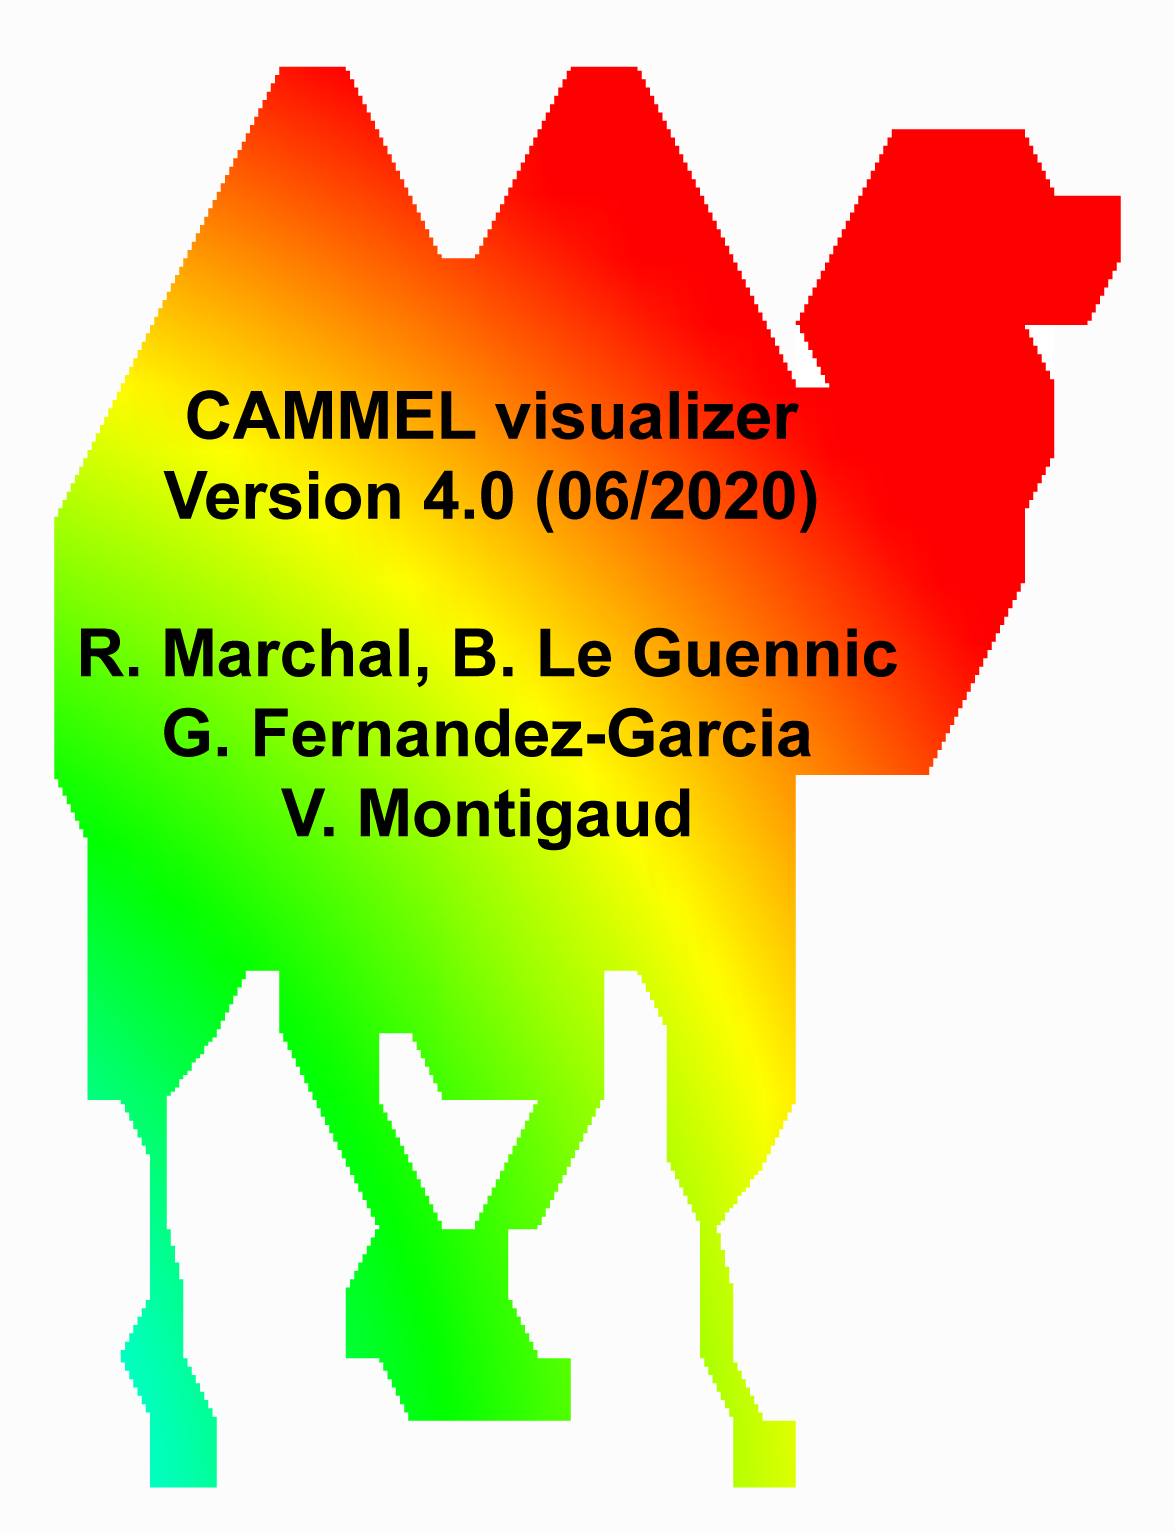
\includegraphics[width=8cm]{cammel_color4.png}\\
\Huge \textbf{The CAlculated Molecular Multipolar ELectrostatics (CAMMEL) software:\\
User guide}
\end{center}
\vspace*{\fill}
\newpage

\tableofcontents

\newpage
\section{Introduction}
\subsection{CAMMEL}
The CAlculated-Molecular Multipolar ELectrostatics (CAMMEL) software is a graphical post-treatment software, interfaced with Molcas and OpenMolcas. Various features are implemented in this software such as:
\begin{itemize}
\item{Wave function decomposition}
\item{Representation of the magnetization curve}
\item{Representation of the Ab initio Transition barriers}
\item{Representation of the susceptibility curve}
\item{Computation and representation of the electrostatic potential surrounding lanthanide atoms}
\end{itemize}

This Software have been developed in the Institut des Sciences Chimiques de Rennes (ISCR UMR CNRS 6226, University of Rennes1) by Rémi Marchal (Computer engineer), Boris Le Guennic (CNRS Research Director), Guglielmo Fernandez-Garcia (PhD) and Vincent Montigaud (PhD).

\subsection{Molcas calculation requirement}
Depending on the CAMMEL features of interest, the Molcas calculation should contains some of the following blocks.

\begin{table}[H]
\begin{center}
\begin{tabular}{|l|c|c|}
\hline
\multirow{2}{*}{CAMMEL feature} & \multicolumn{2}{|c|}{Needed Molcas block} \\
\cline{2-3}
 & SingleAniso & LoProp \\
\hline
Wave function  & x & \\
Magnetization curve & x & \\
Transition barriers & x & \\
Susceptibility curve & x & \\
Electrostatic potential  &  & x \\
\hline
\end{tabular}
\end{center}
\end{table}

\section{Installation}
\subsection{System requirement}
CAMMEL is written in python3 and its graphical part is written in python3 and OpenGl.\\

Therefore, it uses several python library and thus need:
\begin{itemize}
\item{Python3}
\item{The numpy library}
\item{The matplotlib library}
\item{the pyopengl library}
\end{itemize}

\subsection{Installation on Linux}
This recipe is maid for Debian distribution:
\begin{enumerate}
\item{\textbf{Installation of the Python3 interpreter:} sudo apt-get install python3}
\item{\textbf{Installation of pip:} sudo apt-get install python3-pip python3-tk}
\item{\textbf{Installation of the python libraries:} sudo pip3 install numpy matplotlib PyOpenGL opencv-python glfw Pillow}
\end{enumerate}

\subsection{Installation on MacOsX}
For MacOsX, we strongly suggest the use of macport and to follow this recipe:
\begin{enumerate}
\item{\textbf{Install Macport:} see the documentation here: \href{https://www.macports.org/install.php}{https://www.macports.org/install.php}}
\item{\textbf{Install the Python3 interpreter:} sudo /opt/local/bin/port install python36}
\item{\textbf{Install the Python3 libraries:} sudo /opt/local/bin/port install py36-matplotlib py36-numpy py36-opengl py36-pip py36-tkinter}
\item{\textbf{Install the Python3 additional graphical Libraries:} sudo /opt/local/bin/pip3.6 install opencv-python glfw Pillow}
\end{enumerate}

\subsection{Environment variables}
Once the installation is done should define the \$CAMMEL environment variable and append the \$PYTHONPATH using the following command:
\begin{enumerate}
\item{export CAMMEL="location of your CAMMEL directory"}
\item{export PYTHONPATH="location of your CAMMEL directory":\$PYTHONPATH}
\end{enumerate}

\subsection{Launch CAMMEL}
If the installation process finished correctly, you can start CAMMEL using the following command:\\
\textbf{On linux:}python3 \$CAMMEL/CAMMEL.py \\
\textbf{On Mac:}python3.6 \$CAMMEL/CAMMEL.py


\section{How is the electrostatic potential calculated and represented?}
\subsection{Calculation of the potential}
The main feature of CAMMEL is the calculation and the representation of the electrostatic potential surrounding lanthanide atoms.\\

For this purpose, one should first define a radius around the lanthanide. Thus, using this radius, a sphere is considered around the lanthanide ion and a grid (in spherical coordinates) is drawn around this ion. The potential is then calculated on each point of the grid, using the following formula:
\begin{equation}
V(\vec{r_i})=\sum_{at=1}^{N_{at}} \frac{q_{at}}{|\vec{r_{at}}-\vec{r}|} + \frac{\vec{D_{at}}\cdot{}\vec{X_{at}}}{|\vec{r_{at}}-\vec{r_i}|^2} + \frac{\vec{X_{at}}\cdot{}(Q\times\vec{X_{at}})}{2*|\vec{r_i}-\vec{r_{at}}|^3}
\end{equation}
Where $\vec{r_i}$ is the point on which the potential  is calculated, $N_{at}$ the number of atoms of the molecular complex, $\vec{r_{at}}$ the position of each atoms, $q_{at}$ the LoProp charge of atom $at$, $\vec{D_{at}}$ the LoProp dipole of atom $at$, Q the LoProp quadrupole tensor of atom $at$ and $\vec{X_{at}}$ the normalized distance between $i$ and $at$ calculated as:
\begin{equation}
\vec{X_{at}}=\frac{\vec{r_{at}}-\vec{r_i}}{|r_{{at}}-r{i}|}
\end{equation}

\textbf{Please not that all the atom of the molecule is considered for computing the potential except the lanthanide atom around which the potential is calculated.}

\subsection{Representation of the potential}
The calculated potential is then represented in 2 different ways, depending on the user choice:
\begin{enumerate}
\item{on a sphere}
\item{on a \og potential surface \fg{} } 
\end{enumerate}
\subsubsection{On a sphere}
The potential surface is in this case represented as a sphere and the color-map is given by the values of the potential.
\subsubsection{On a \og potential surface \fg{}}
The grid in spherical coordinates is in this case readjusted, changing the $r$  coordinate of each grid point with regard to the value of the potential at this point. The color-map is given by the values of the potential. In this case, we have redundancy of the representation of the potential since they are represented by the color-map but also by the height of the irregularities of the surface. However, even if this redundancy can appear as not necessary, it strongly helps if the molecular complex shows strong anisotropy.
\subsubsection{Other features of the representation of the potential}
CAMMEL allows also to map not only the full potential but also each of its contribution (by the monopoles, dipoles and quadrupoles). It also give you the ability of showing the molecule and the orientation of the g tensors.
\section{Citation and contact}
\subsection{Citation}
If you publish some results from CAMMEL, please cite the following paper:\\

\textit{Magnetic Slow Relaxation in a Metal–Organic Framework Made of Chains of Ferromagnetically Coupled Single-Molecule Magnets}, G. Huang,G. Fernandez-Garcia,I. Badiane, M. Camarra, S. Freslon, O. Guillou, C. Daiguebonne, F. Totti, O. Cador, T. Guizouarn, B. Le Guennic, K. Bernot, \textbf{Chem. Eur. J.}, 2018, 24, 6983


\subsection{Contact}
Please contact Boris (boris.leguennic@univ-rennes1.fr) for scientific support and Rémi (remi.marchal@univ-rennes1.fr) for technical support.

\end{document}